\subsection{Aufstieg von Luftblasen}
	\subsubsection{Dichte des Spülmittels}
		Nach dem Archimedischen Prinzip ist die Auftriebskraft, die die Flasche ins Wasser hält, gleich die Gewicht des verdrängten Wasser. Somit gilt:
		\begin{equation}
			F_A = \rho_\wasser V_\wasser g
		\end{equation}
		Da die Flasche im Wasser schwimmt, also ist die Flasche im Gleichgewicht und es gilt:
		\begin{align}
			F_G &= F_A \\
			\rho_\spuli V_\spuli \cancel{g} &= \rho_\wasser V_\wasser \cancel{g} \\
			\rho_\spuli &= \rho_\wasser \frac{V_\wasser}{V_\spuli}
		\end{align}
		Dabei ist die Volumen des verdrängtes Wasser als $V_\wasser = \SI{650(50)}{\centi\meter\cubed}$.

		\begin{wrapfigure}{o}{0.4\textwidth}
			\centering
			\vspace{-1em}
			\captionsetup{width=0.4\textwidth, justification=centering}
			\includegraphics[width=0.25\textwidth]{tv1-dichte-auswertung.png}
			\caption{Messungen der Höhe des Wasserpegels in \tracker{}}
			\vspace{-3em}
		\end{wrapfigure}
		Wir nehmen an, dass der Flasche die Querschnittsfläche für den unteren Teil überall gleich ist, somit ist das Volumen proportional zur Höhe und wir erhalten:
		\begin{align}
			\rho_\spuli &= \rho_\wasser \frac{h_\wasser}{h_\spuli}
		\end{align}
		mit dem entsprechen Fehler:
		\begin{align}
			\Delta \rho_\spuli = \rho_\spuli \relquad{h_\wasser,h_\spuli}
		\end{align}
		Aus \tracker{} und The Engineering Toolbox\footnote{\url{www.engineeringtoolbox.com/water-density-specific-weight-d\_595.html?vA=29&units=C\#}} haben wir als Werten:
		\begin{equation*}
			\begin{tabu}{llr}
				\toprule
				\text{Höhe des Wasserpegels} & h_\wasser & \SI{0.160(5)}{\meter} \\
				\text{Höhe des Spülmittels} & h_\spuli & \SI{0.147(5)}{\meter} \\
				\text{Wasserdichte bei \SI{29}{\celsius}} & \rho_\wasser & \SI{995.96}{\kilo\gram\per\meter\cubed} \\
				\bottomrule
			\end{tabu}
		\end{equation*}
		Damit gilt:
		\begin{align}
			\rho_\spuli &= \SI{995.96}{\kilo\gram\per\meter\cubed} \frac{\SI{0.160}{\meter}}{\SI{0.147}{\meter} }
			= \SI{1084.04}{\kilo\gram\per\meter\cubed} \sigfig{6} \\
			\Delta \rho &= \SI{995.96}{\kilo\gram\per\meter\cubed} \frac{\SI{0.160}{\meter}}{\SI{0.147}{\meter} } 
			\sqrt{\left( \frac{\SI{0.005}{\meter}}{\SI{0.160}{\meter}} \right)^2 + \left( \frac{\SI{0.005}{\meter}}{\SI{0.147}{\meter}} \right)^2} 
			= \SI{50.0714}{\kilo\gram\per\meter\cubed} \sigfig{6}
		\end{align}
		Folglich haben wir eine Dichte von $\rho_\spuli = \SI{1080(60)}{\kilo\gram\per\meter\cubed} = \SI{1.08(6)}{\gram\per\centi\meter\cubed}$.
		\newpage
		Im Vergleich zum Literaturwert\footnote{\url{daten.oehme-lorito.de/sdb/frosch\%20geschirrsp\%C3\%BClmittel\%20limonen.pdf}, Seite 6} haben wir:
		\begin{center}
			\begin{tabular}{lrr}
				\toprule
				Quelle & Temperatur & Wert$/\si{\gram\per\centi\meter\cubed}$ \\
				\midrule
				Experiment & \SI{29(1)}{\celsius}& \num{1.08(6)} \\
				Aräometer   & $\approx$ \SI{23}{\celsius} & \num{1.024(1)} \\
				Hersteller & \SI{20}{\celsius} & \num{1.025} \\
				\bottomrule
			\end{tabular}
		\end{center}
		Die von Aräometer ermittelte Dichte stimmt mit dem Literaturwert überein. Unser experimenteller Wert ist aber nur verträglich mit der anderen zwei Werten. Dieser Unterschied liegt vermutlich daran, dass das Gewicht der Flasche nicht berücksichtigt war. Am Boden der Flasche gibt es auch eine Aussparung, was auch nicht berücksichtigt war. 

	\newpage
	\subsubsection{Viskosität des warmen Spülmittels}
		Die Aufnahmen wurden erst mit \texttt{ffmpeg} geschnittet, bevor sie im \tracker{} geladen sind. Dadurch ist die Anzahl der Frames für jeden Verlauf niedrig gehalten und \tracker{} kann somit schneller die Videos verarbeiten.

		Zur Messung des Durchmessers $2r$ wurden $5$ Messungen mit der "Measuring Tape" Funktion in \tracker{} durchgeführt. Der Mittelwert und die Standardabweichung wurden dann mit LibreOffice Calc berechnet. Dazu sind die Funktionen \texttt{AVERAGE} und \texttt{STDEV} verwendet. Die Standardabweichung entspricht dann die Unsicherheit des Durchmessers:
		\begin{center}
			\begin{tabular}{l*{6}{r}}
				\toprule
				Blase & $2r_1/\si{\milli\meter}$ & $2r_2/\si{\milli\meter}$ & $2r_3/\si{\milli\meter}$ & $2r_4/\si{\milli\meter}$ & $2r_5/\si{\milli\meter}$ & $\overline{(2r)}/\si{\milli\meter}$ \\
				\midrule
				\num{1} & \num{2.753} & \num{2.810} & \num{2.890} & \num{2.814} & \num{2.920}  & \num{2.84(7)} \\
				\num{2} & \num{2.664} & \num{2.629} & \num{2.632} & \num{2.593} & \num{2.645}  & \num{2.633(27)} \\
				\num{3} & \num{3.033} & \num{3.073} & \num{3.014} & \num{2.973} & \num{3.117}  & \num{3.04(6)} \\
				\num{4} & \num{2.675} & \num{2.769} & \num{2.725} & \num{2.501} & \num{2.545}  & \num{2.64(12)} \\
				\num{5} & \num{3.423} & \num{3.463} & \num{3.539} & \num{3.547} & \num{3.502}  & \num{3.49(6)} \\
				\num{6} & \num{3.537} & \num{3.586} & \num{3.597} & \num{3.501} & \num{3.595}  & \num{3.56(5)} \\
				\num{7} & \num{7.351} & \num{6.899} & \num{6.953} & \num{7.407} & \num{6.916}  & \num{7.11(26)} \\
				\num{8} & \num{5.511} & \num{5.774} & \num{5.368} & \num{5.721} & \num{5.472}  & \num{5.57(18)} \\
				\num{9} & \num{2.939} & \num{2.640} & \num{2.693} & \num{2.724} & \num{2.770}  & \num{2.75(12)} \\
				\num{10} & \num{3.641} & \num{3.797} & \num{3.858} & \num{3.733} & \num{3.668} & \num{3.74(9)} \\
				\bottomrule
			\end{tabular}
		\end{center}

		Die erhaltene Zeit-Position Daten aus \tracker{} sind mit \gnuplot{} geplottet und es wurde eine Kurveanpassung zur $y = mt + c~$ für jede Blase durchgeführt. Da \tracker{} keine explizite Unsicherheit ermittelt, vernachlässigen wir sie für die Kurvenanpassung.

		Für das genaue \gnuplot{} Code, siehe Appendix \ref{appdx:tvone-warm}. 
		% https://tex.stackexchange.com/a/98142
		\begin{figure}[H]
			\centering
			\captionsetup{width=0.8\textwidth, justification=centering}
			\resizebox{\linewidth}{!}{% GNUPLOT: LaTeX picture with Postscript
\begingroup
  \makeatletter
  \providecommand\color[2][]{%
    \GenericError{(gnuplot) \space\space\space\@spaces}{%
      Package color not loaded in conjunction with
      terminal option `colourtext'%
    }{See the gnuplot documentation for explanation.%
    }{Either use 'blacktext' in gnuplot or load the package
      color.sty in LaTeX.}%
    \renewcommand\color[2][]{}%
  }%
  \providecommand\includegraphics[2][]{%
    \GenericError{(gnuplot) \space\space\space\@spaces}{%
      Package graphicx or graphics not loaded%
    }{See the gnuplot documentation for explanation.%
    }{The gnuplot epslatex terminal needs graphicx.sty or graphics.sty.}%
    \renewcommand\includegraphics[2][]{}%
  }%
  \providecommand\rotatebox[2]{#2}%
  \@ifundefined{ifGPcolor}{%
    \newif\ifGPcolor
    \GPcolortrue
  }{}%
  \@ifundefined{ifGPblacktext}{%
    \newif\ifGPblacktext
    \GPblacktexttrue
  }{}%
  % define a \g@addto@macro without @ in the name:
  \let\gplgaddtomacro\g@addto@macro
  % define empty templates for all commands taking text:
  \gdef\gplbacktext{}%
  \gdef\gplfronttext{}%
  \makeatother
  \ifGPblacktext
    % no textcolor at all
    \def\colorrgb#1{}%
    \def\colorgray#1{}%
  \else
    % gray or color?
    \ifGPcolor
      \def\colorrgb#1{\color[rgb]{#1}}%
      \def\colorgray#1{\color[gray]{#1}}%
      \expandafter\def\csname LTw\endcsname{\color{white}}%
      \expandafter\def\csname LTb\endcsname{\color{black}}%
      \expandafter\def\csname LTa\endcsname{\color{black}}%
      \expandafter\def\csname LT0\endcsname{\color[rgb]{1,0,0}}%
      \expandafter\def\csname LT1\endcsname{\color[rgb]{0,1,0}}%
      \expandafter\def\csname LT2\endcsname{\color[rgb]{0,0,1}}%
      \expandafter\def\csname LT3\endcsname{\color[rgb]{1,0,1}}%
      \expandafter\def\csname LT4\endcsname{\color[rgb]{0,1,1}}%
      \expandafter\def\csname LT5\endcsname{\color[rgb]{1,1,0}}%
      \expandafter\def\csname LT6\endcsname{\color[rgb]{0,0,0}}%
      \expandafter\def\csname LT7\endcsname{\color[rgb]{1,0.3,0}}%
      \expandafter\def\csname LT8\endcsname{\color[rgb]{0.5,0.5,0.5}}%
    \else
      % gray
      \def\colorrgb#1{\color{black}}%
      \def\colorgray#1{\color[gray]{#1}}%
      \expandafter\def\csname LTw\endcsname{\color{white}}%
      \expandafter\def\csname LTb\endcsname{\color{black}}%
      \expandafter\def\csname LTa\endcsname{\color{black}}%
      \expandafter\def\csname LT0\endcsname{\color{black}}%
      \expandafter\def\csname LT1\endcsname{\color{black}}%
      \expandafter\def\csname LT2\endcsname{\color{black}}%
      \expandafter\def\csname LT3\endcsname{\color{black}}%
      \expandafter\def\csname LT4\endcsname{\color{black}}%
      \expandafter\def\csname LT5\endcsname{\color{black}}%
      \expandafter\def\csname LT6\endcsname{\color{black}}%
      \expandafter\def\csname LT7\endcsname{\color{black}}%
      \expandafter\def\csname LT8\endcsname{\color{black}}%
    \fi
  \fi
    \setlength{\unitlength}{0.0500bp}%
    \ifx\gptboxheight\undefined%
      \newlength{\gptboxheight}%
      \newlength{\gptboxwidth}%
      \newsavebox{\gptboxtext}%
    \fi%
    \setlength{\fboxrule}{0.5pt}%
    \setlength{\fboxsep}{1pt}%
\begin{picture}(10080.00,5760.00)%
    \gplgaddtomacro\gplbacktext{%
      \csname LTb\endcsname%%
      \put(946,704){\makebox(0,0)[r]{\strut{}$-100$}}%
      \put(946,1104){\makebox(0,0)[r]{\strut{}$0$}}%
      \put(946,1503){\makebox(0,0)[r]{\strut{}$100$}}%
      \put(946,1903){\makebox(0,0)[r]{\strut{}$200$}}%
      \put(946,2302){\makebox(0,0)[r]{\strut{}$300$}}%
      \put(946,2702){\makebox(0,0)[r]{\strut{}$400$}}%
      \put(946,3101){\makebox(0,0)[r]{\strut{}$500$}}%
      \put(946,3501){\makebox(0,0)[r]{\strut{}$600$}}%
      \put(946,3900){\makebox(0,0)[r]{\strut{}$700$}}%
      \put(946,4300){\makebox(0,0)[r]{\strut{}$800$}}%
      \put(946,4699){\makebox(0,0)[r]{\strut{}$900$}}%
      \put(946,5099){\makebox(0,0)[r]{\strut{}$1000$}}%
      \put(1078,484){\makebox(0,0){\strut{}$0$}}%
      \put(1939,484){\makebox(0,0){\strut{}$1$}}%
      \put(2799,484){\makebox(0,0){\strut{}$2$}}%
      \put(3660,484){\makebox(0,0){\strut{}$3$}}%
      \put(4520,484){\makebox(0,0){\strut{}$4$}}%
      \put(5381,484){\makebox(0,0){\strut{}$5$}}%
      \put(6241,484){\makebox(0,0){\strut{}$6$}}%
      \put(7102,484){\makebox(0,0){\strut{}$7$}}%
      \put(7962,484){\makebox(0,0){\strut{}$8$}}%
      \put(8823,484){\makebox(0,0){\strut{}$9$}}%
      \put(9683,484){\makebox(0,0){\strut{}$10$}}%
    }%
    \gplgaddtomacro\gplfronttext{%
      \csname LTb\endcsname%%
      \put(209,2901){\rotatebox{-270}{\makebox(0,0){\strut{}Vertikale Position $y/\si{\milli\meter}$}}}%
      \put(5380,154){\makebox(0,0){\strut{}Zeit $t/\si{\second}$}}%
      \csname LTb\endcsname%%
      \put(5993,4926){\makebox(0,0)[r]{\strut{}Blase 1}}%
      \csname LTb\endcsname%%
      \put(5993,4706){\makebox(0,0)[r]{\strut{}Blase 2}}%
      \csname LTb\endcsname%%
      \put(5993,4486){\makebox(0,0)[r]{\strut{}Blase 3}}%
      \csname LTb\endcsname%%
      \put(5993,4266){\makebox(0,0)[r]{\strut{}Blase 4}}%
      \csname LTb\endcsname%%
      \put(5993,4046){\makebox(0,0)[r]{\strut{}Blase 5}}%
      \csname LTb\endcsname%%
      \put(5993,3826){\makebox(0,0)[r]{\strut{}Blase 6}}%
      \csname LTb\endcsname%%
      \put(5993,3606){\makebox(0,0)[r]{\strut{}Blase 7}}%
      \csname LTb\endcsname%%
      \put(5993,3386){\makebox(0,0)[r]{\strut{}Blase 8}}%
      \csname LTb\endcsname%%
      \put(5993,3166){\makebox(0,0)[r]{\strut{}Blase 9}}%
      \csname LTb\endcsname%%
      \put(5993,2946){\makebox(0,0)[r]{\strut{}Blase 10}}%
      \csname LTb\endcsname%%
      \put(8696,4926){\makebox(0,0)[r]{\strut{}$18,75936t + (0,83453)$}}%
      \csname LTb\endcsname%%
      \put(8696,4706){\makebox(0,0)[r]{\strut{}$14,88056t + (0,39407)$}}%
      \csname LTb\endcsname%%
      \put(8696,4486){\makebox(0,0)[r]{\strut{}$23,80945t + (0,10412)$}}%
      \csname LTb\endcsname%%
      \put(8696,4266){\makebox(0,0)[r]{\strut{}$14,78785t + (-1,55167)$}}%
      \csname LTb\endcsname%%
      \put(8696,4046){\makebox(0,0)[r]{\strut{}$28,05332t + (-2,10395)$}}%
      \csname LTb\endcsname%%
      \put(8696,3826){\makebox(0,0)[r]{\strut{}$35,18369t + (1,75442)$}}%
      \csname LTb\endcsname%%
      \put(8696,3606){\makebox(0,0)[r]{\strut{}$99,39234t + (0,47523)$}}%
      \csname LTb\endcsname%%
      \put(8696,3386){\makebox(0,0)[r]{\strut{}$67,19169t + (1,10226)$}}%
      \csname LTb\endcsname%%
      \put(8696,3166){\makebox(0,0)[r]{\strut{}$17,52108t + (-0,18687)$}}%
      \csname LTb\endcsname%%
      \put(8696,2946){\makebox(0,0)[r]{\strut{}$36,19531t + (0,01841)$}}%
      \csname LTb\endcsname%%
      \put(5380,5429){\makebox(0,0){\strut{}Aufstiegsverlauf der Blasen (Warm)}}%
    }%
    \gplbacktext
    \put(0,0){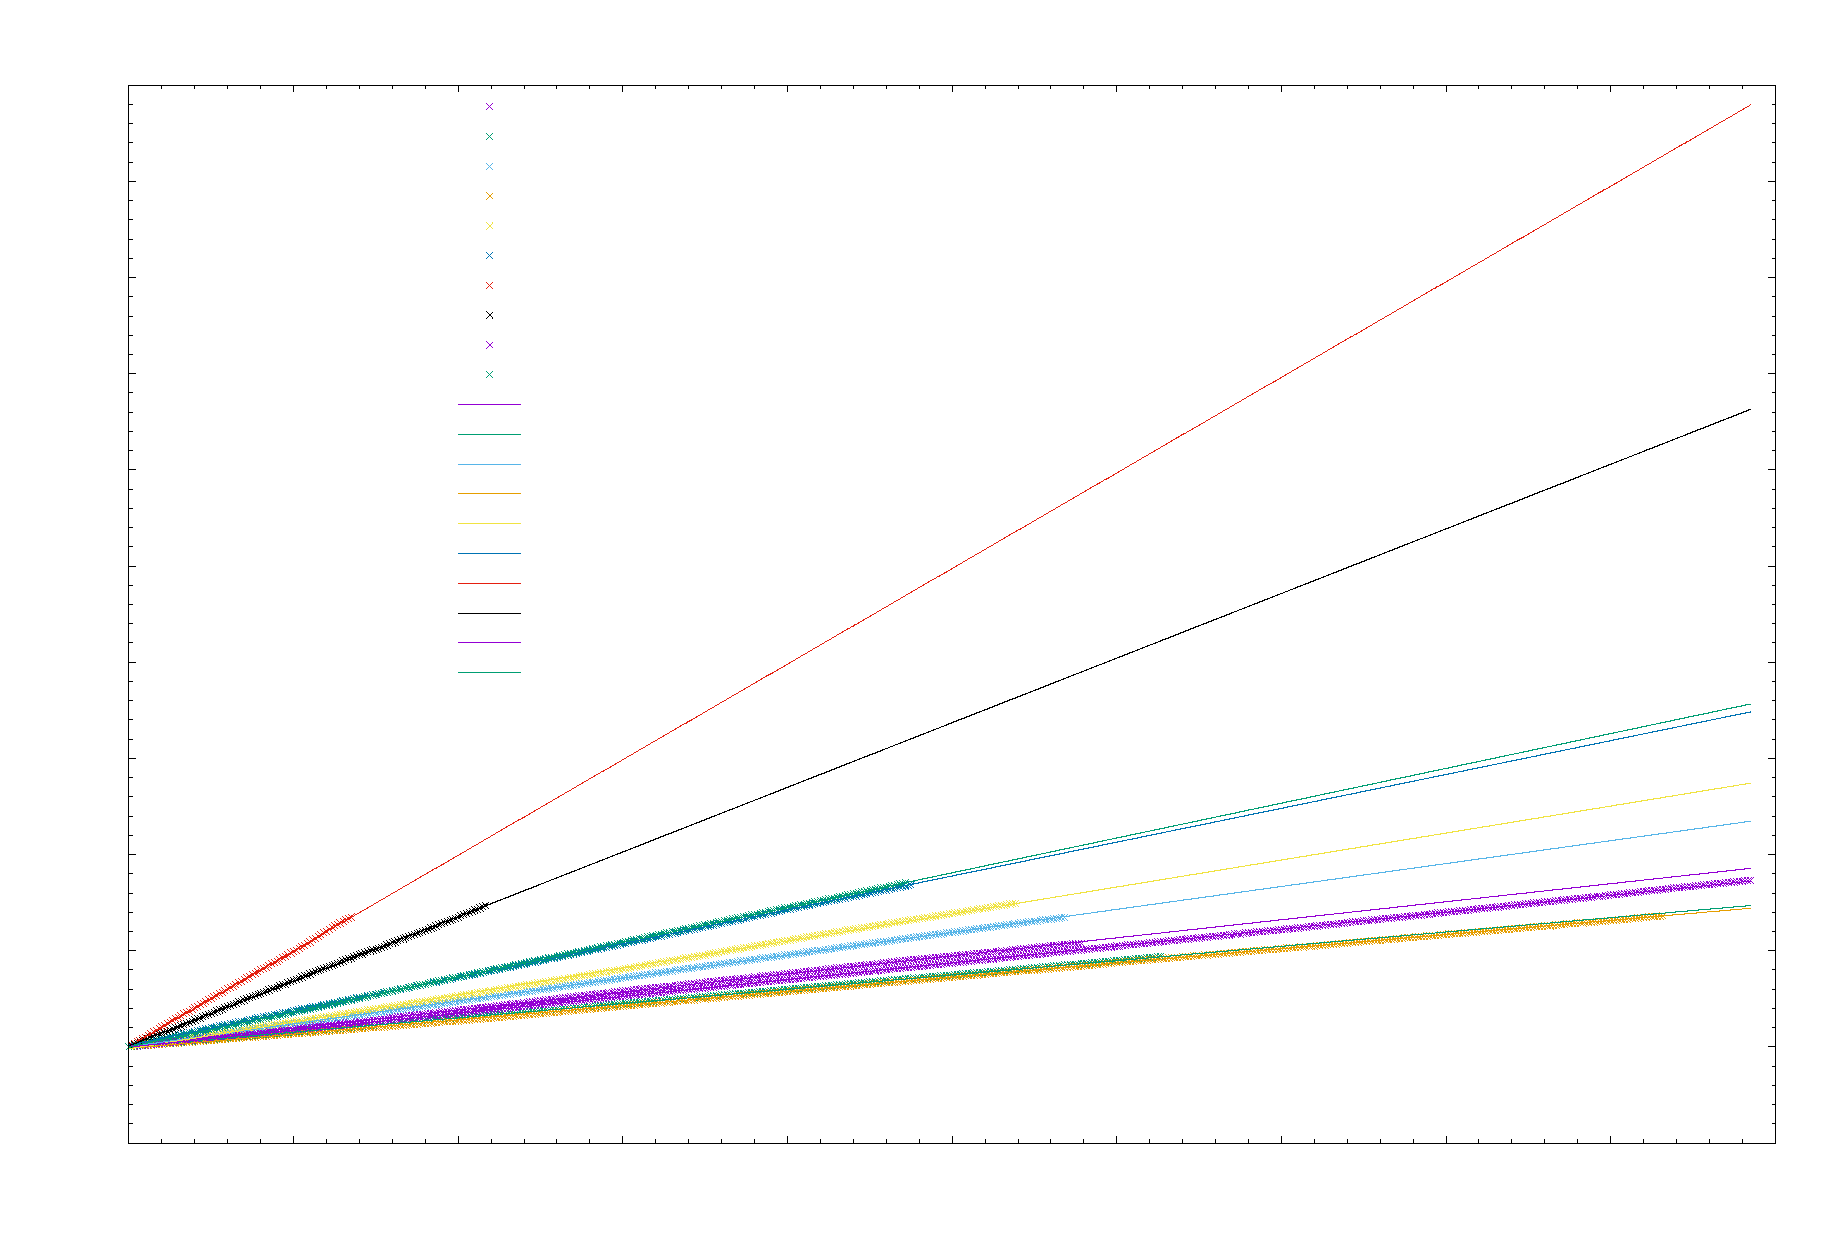
\includegraphics[width={504.00bp},height={288.00bp}]{tv1-plot-warm}}%
    \gplfronttext
  \end{picture}%
\endgroup
}
			\caption{Aufstieg der Luftblasen im warmen Spülmittel \textattachfile[author={Yudong Sun},color={0 0.404 0.584},description={.zip Datei mit der Messwerten},mimetype={application/zip},timezone={+02'00'}]{./attachments/luftblasen-warm.zip}{\textit{(Daten)}}}
			\vspace{-1em}
		\end{figure}
		Als Endergebnis erhalten wir:
		\begin{center}
			\begin{tabular}{lrrr}
				\toprule
				Blase Nr. & $m/\si{\milli\meter\per\second}$ & $c/\si{\milli\meter}$ & $\chi^2_\text{red}$ \\
				\midrule
					$1$ &  \num{18,75936(1679)} & \num{0,83453(5611)} & \num{0,27505} \\
					$2$ &  \num{14,88056(310)} & \num{0,39407(1123)} & \num{0,01194} \\
					$3$ &  \num{23,80945(1052)} & \num{0,10412(3453)} & \num{0,10242} \\
					$4$ &  \num{14,78785(770)} & \num{-1,55167(4144)} & \num{0,24111} \\
					$5$ &  \num{28,05332(3272)} & \num{-2,10395(10176)} & \num{0,84266} \\
					$6$ &  \num{35,18369(1851)} & \num{1,75442(5080)} & \num{0,18549} \\
					$7$ &  \num{99,39234(14013)} & \num{0,47523(10955)} & \num{0,25057} \\
					$8$ &  \num{67,19169(8685)} & \num{1,10226(10885)} & \num{0,39251} \\
					$9$ &  \num{17,52108(486)} & \num{-0,18687(2767)} & \num{0,11364} \\
					$10$ & \num{36,19531(880)} & \num{0,01841(2399)} & \num{0,04108} \\
				\bottomrule
			\end{tabular}
		\end{center}
		Aus der niedrigen $\chi^2_\text{red}$ sind alle Kurveanpassungen gut. $m$ entspricht in diesem Fall die Geschwindigkeit $v$.
		Laut der Anleitung gilt:
		\begin{align}
			\eta_\spuli &= \frac{2\cdot g\rho_\spuli}{9\cdot v_\text{Luftblase}}\cdot r^2_\text{Luftblase} = \frac{g\cdot \rho_\spuli}{18\cdot v_\text{Luftblase}}\cdot (2r_\text{Luftblase})^2 \label{eqn:warm-eta} \\
			\Delta \eta_\spuli &= \eta_\spuli \sqrt{
				\left(\frac{\Delta \rho_\spuli}{\rho_\spuli}\right)^2 +
				\left(\frac{\Delta v_\text{Luftblase}}{v_\text{Luftblase}}\right)^2 +
				\left(2\frac{\Delta (2r_\text{Luftblase})}{2r_\text{Luftblase}}\right)^2
			} \label{eqn:warm-delta-eta}
		\end{align}
		Die Viskositäten und die entsprechenden Fehler wurden dann mittels LibreOffice Calc anhand \eqref{eqn:warm-eta} und \eqref{eqn:warm-delta-eta} berechnet. Die genaue Rechnung sind wegen Übersichtlichkeit hier ausgelassen.

		Als Ergebnis erhalten wir:
		\begin{center}
			\begin{tabular}{lrrr}
				\toprule
				Blase Nr. $i$ & $2r_i/\si{\milli\meter}$ & $v_i/\si{\milli\meter\per\second}$ & $\eta_i/\si{\milli\pascal\second}$ \\
				\midrule
				\num{1} & \num{2.84(7)} & \num{18.759(17)} & \num{253(19)} \\
				\num{2} & \num{2.633(27)} & \num{14.881(4)} & \num{274(17)} \\
				\num{3} & \num{3.04(6)} & \num{23.809(11)} & \num{228(16)} \\
				\num{4} & \num{2.64(12)} & \num{14.788(8)} & \num{280(30)} \\
				\num{5} & \num{3.49(6)} & \num{28.05(4)} & \num{256(17)} \\
				\num{6} & \num{3.56(5)} & \num{35.18(2)} & \num{212(14)} \\
				\num{7} & \num{7.11(26)} & \num{99.39(15)} & \num{299(28)} \\
				\num{8} & \num{5.57(18)} & \num{67.19(9)} & \num{272(24)} \\
				\num{9} & \num{2.75(12)} & \num{17.521(5)} & \num{254(27)} \\
				\num{10} & \num{3.74(9)} & \num{36.195(9)} & \num{227(17)} \\
				\bottomrule
			\end{tabular}
		\end{center}
		Der Mittelwert $\overline{\eta}$ ist dann gegeben durch:
		\begin{align}
			\overline{\eta} = \frac{1}{10}\sum^{10}_{i=1}\eta_i  && \text{mit} && \Delta \overline{\eta} = \frac{1}{10} \sqrt{\sum^{10}_{i=1}(\Delta\eta_i)^2} \label{eqn:avg-eta-warm}
		\end{align}
		und die Standardabweichung:
		\begin{align}
			s(\eta) = \sqrt{\frac{1}{10 - 1} \sum^{10}_{i=1}(\eta_i - \overline{\eta})^2}
			\label{eqn:stdev-eta-warm}
		\end{align}
		Die genaue Rechnungen erfolgen anhand \eqref{eqn:avg-eta-warm} und \eqref{eqn:stdev-eta-warm} in LibreOffice Calc und sind wegen Über\-sicht\-lich\-keit hier ausgelassen. Für den Mittelwert und die Standabweichung sind die Funktionen \texttt{AVERAGE} und \texttt{STDEV.S} direkt verwendet. Wir erhalten:
		\begin{center}
			\begin{tabular}{lrr}
				\toprule
				Mittelwert & $\overline{\eta}$ & \SI{255.5}{\milli\pascal\second}\\
				Unsicherheit des Mittelwertes & $\Delta\overline{\eta}$ & \SI{6.9}{\milli\pascal\second}\\
				Standardabweichung & $s(\eta)$ & \SI{28}{\milli\pascal\second}\\
				\bottomrule
			\end{tabular}
		\end{center}
		wobei $\Delta\overline{\eta}$ und $s(\eta)$ beides auf 2 signifikanten Ziffern aufgerundet sind. 

		Da die Standardabweichung größer als die Unsicherheit des Mittelwertes ist, nehmen wir die Standardabweichung als Fehler und erhalten für $T = \SI{29(1)}{\celsius}$ eine Viskosität von $\eta = \SI{256(28)}{\milli\pascal\second}$.

	\newpage
	\subsubsection{Viskosität des kalten Spülmittels}
		Wir wiederholen nun alle Rechnungen für das kalte Spülmittel. Sodass die Variablen nicht durcheinander kommen, sind die Auswertung zum kalten Spülmittel hier im zweiten Abschnitt geteilt. 

		Es ist davon ausgegangen, dass die Dichte des Spülmittels nicht Temperaturabhängig ist.

		\iu{Messung der Durchmesser}

		Im Allgemein sind die Durchmesser für das kalte Spülmittel größer, da es schwieriger war, eine Blase im Spülmittel zu pusten.
		\begin{center}
			\begin{tabular}{l*{6}{r}}
				\toprule
				Blase & $2r_1/\si{\milli\meter}$ & $2r_2/\si{\milli\meter}$ & $2r_3/\si{\milli\meter}$ & $2r_4/\si{\milli\meter}$ & $2r_5/\si{\milli\meter}$ & $\overline{(2r)}/\si{\milli\meter}$ \\
				\midrule
				\num{1} & \num{8.164} & \num{8.244} & \num{8.149} & \num{8.256} & \num{8.284} & \num{8.23(6)} \\
				\num{2} & \num{8.082} & \num{8.039} & \num{8.067} & \num{8.107} & \num{7.993} & \num{8.05(5)} \\
				\num{3} & \num{11.80} & \num{12.01} & \num{12.11} & \num{11.54} & \num{11.99} & \num{11.91(26)} \\
				\num{4} & \num{13.50} & \num{13.46} & \num{13.70} & \num{14.09} & \num{13.66} & \num{13.73(27)} \\
				\num{5} & \num{8.508} & \num{8.550} & \num{8.663} & \num{8.466} & \num{8.497} & \num{8.54(9)} \\
				\num{6} & \num{9.846} & \num{9.806} & \num{9.702} & \num{9.746} & \num{9.798} & \num{9.76(5)} \\
				\num{7} & \num{10.74} & \num{10.90} & \num{10.76} & \num{10.94} & \num{10.82} & \num{10.86(9)} \\
				\num{8} & \num{8.979} & \num{8.913} & \num{9.058} & \num{8.873} & \num{8.892} & \num{8.93(9)} \\
				\num{9} & \num{9.062} & \num{9.031} & \num{8.886} & \num{9.133} & \num{9.042} & \num{9.02(11)} \\
				\num{10} & \num{8.966} & \num{9.070} & \num{9.082} & \num{9.053} & \num{9.173} & \num{9.09(6)} \\
				\bottomrule
			\end{tabular}
		\end{center}
		\iu{Geschwindigkeit mittels \gnuplot{}}

		Für das genaue \gnuplot{} Code, siehe Appendix \ref{appdx:tvone-cold}. 
		% https://tex.stackexchange.com/a/98142
		\begin{figure}[H]
			\centering
			\captionsetup{width=0.8\textwidth, justification=centering}
			\resizebox{\linewidth}{!}{% GNUPLOT: LaTeX picture with Postscript
\begingroup
  \makeatletter
  \providecommand\color[2][]{%
    \GenericError{(gnuplot) \space\space\space\@spaces}{%
      Package color not loaded in conjunction with
      terminal option `colourtext'%
    }{See the gnuplot documentation for explanation.%
    }{Either use 'blacktext' in gnuplot or load the package
      color.sty in LaTeX.}%
    \renewcommand\color[2][]{}%
  }%
  \providecommand\includegraphics[2][]{%
    \GenericError{(gnuplot) \space\space\space\@spaces}{%
      Package graphicx or graphics not loaded%
    }{See the gnuplot documentation for explanation.%
    }{The gnuplot epslatex terminal needs graphicx.sty or graphics.sty.}%
    \renewcommand\includegraphics[2][]{}%
  }%
  \providecommand\rotatebox[2]{#2}%
  \@ifundefined{ifGPcolor}{%
    \newif\ifGPcolor
    \GPcolortrue
  }{}%
  \@ifundefined{ifGPblacktext}{%
    \newif\ifGPblacktext
    \GPblacktexttrue
  }{}%
  % define a \g@addto@macro without @ in the name:
  \let\gplgaddtomacro\g@addto@macro
  % define empty templates for all commands taking text:
  \gdef\gplbacktext{}%
  \gdef\gplfronttext{}%
  \makeatother
  \ifGPblacktext
    % no textcolor at all
    \def\colorrgb#1{}%
    \def\colorgray#1{}%
  \else
    % gray or color?
    \ifGPcolor
      \def\colorrgb#1{\color[rgb]{#1}}%
      \def\colorgray#1{\color[gray]{#1}}%
      \expandafter\def\csname LTw\endcsname{\color{white}}%
      \expandafter\def\csname LTb\endcsname{\color{black}}%
      \expandafter\def\csname LTa\endcsname{\color{black}}%
      \expandafter\def\csname LT0\endcsname{\color[rgb]{1,0,0}}%
      \expandafter\def\csname LT1\endcsname{\color[rgb]{0,1,0}}%
      \expandafter\def\csname LT2\endcsname{\color[rgb]{0,0,1}}%
      \expandafter\def\csname LT3\endcsname{\color[rgb]{1,0,1}}%
      \expandafter\def\csname LT4\endcsname{\color[rgb]{0,1,1}}%
      \expandafter\def\csname LT5\endcsname{\color[rgb]{1,1,0}}%
      \expandafter\def\csname LT6\endcsname{\color[rgb]{0,0,0}}%
      \expandafter\def\csname LT7\endcsname{\color[rgb]{1,0.3,0}}%
      \expandafter\def\csname LT8\endcsname{\color[rgb]{0.5,0.5,0.5}}%
    \else
      % gray
      \def\colorrgb#1{\color{black}}%
      \def\colorgray#1{\color[gray]{#1}}%
      \expandafter\def\csname LTw\endcsname{\color{white}}%
      \expandafter\def\csname LTb\endcsname{\color{black}}%
      \expandafter\def\csname LTa\endcsname{\color{black}}%
      \expandafter\def\csname LT0\endcsname{\color{black}}%
      \expandafter\def\csname LT1\endcsname{\color{black}}%
      \expandafter\def\csname LT2\endcsname{\color{black}}%
      \expandafter\def\csname LT3\endcsname{\color{black}}%
      \expandafter\def\csname LT4\endcsname{\color{black}}%
      \expandafter\def\csname LT5\endcsname{\color{black}}%
      \expandafter\def\csname LT6\endcsname{\color{black}}%
      \expandafter\def\csname LT7\endcsname{\color{black}}%
      \expandafter\def\csname LT8\endcsname{\color{black}}%
    \fi
  \fi
    \setlength{\unitlength}{0.0500bp}%
    \ifx\gptboxheight\undefined%
      \newlength{\gptboxheight}%
      \newlength{\gptboxwidth}%
      \newsavebox{\gptboxtext}%
    \fi%
    \setlength{\fboxrule}{0.5pt}%
    \setlength{\fboxsep}{1pt}%
\begin{picture}(10080.00,6480.00)%
    \gplgaddtomacro\gplbacktext{%
      \csname LTb\endcsname%%
      \put(814,704){\makebox(0,0)[r]{\strut{}$-50$}}%
      \put(814,1435){\makebox(0,0)[r]{\strut{}$0$}}%
      \put(814,2165){\makebox(0,0)[r]{\strut{}$50$}}%
      \put(814,2896){\makebox(0,0)[r]{\strut{}$100$}}%
      \put(814,3627){\makebox(0,0)[r]{\strut{}$150$}}%
      \put(814,4358){\makebox(0,0)[r]{\strut{}$200$}}%
      \put(814,5088){\makebox(0,0)[r]{\strut{}$250$}}%
      \put(814,5819){\makebox(0,0)[r]{\strut{}$300$}}%
      \put(946,484){\makebox(0,0){\strut{}$0$}}%
      \put(2038,484){\makebox(0,0){\strut{}$1$}}%
      \put(3130,484){\makebox(0,0){\strut{}$2$}}%
      \put(4222,484){\makebox(0,0){\strut{}$3$}}%
      \put(5315,484){\makebox(0,0){\strut{}$4$}}%
      \put(6407,484){\makebox(0,0){\strut{}$5$}}%
      \put(7499,484){\makebox(0,0){\strut{}$6$}}%
      \put(8591,484){\makebox(0,0){\strut{}$7$}}%
      \put(9683,484){\makebox(0,0){\strut{}$8$}}%
    }%
    \gplgaddtomacro\gplfronttext{%
      \csname LTb\endcsname%%
      \put(209,3261){\rotatebox{-270}{\makebox(0,0){\strut{}Vertikale Position $y/\si{\milli\meter}$}}}%
      \put(5314,154){\makebox(0,0){\strut{}Zeit $t/\si{\second}$}}%
      \csname LTb\endcsname%%
      \put(5993,5646){\makebox(0,0)[r]{\strut{}Blase 1}}%
      \csname LTb\endcsname%%
      \put(5993,5426){\makebox(0,0)[r]{\strut{}Blase 2}}%
      \csname LTb\endcsname%%
      \put(5993,5206){\makebox(0,0)[r]{\strut{}Blase 3}}%
      \csname LTb\endcsname%%
      \put(5993,4986){\makebox(0,0)[r]{\strut{}Blase 4}}%
      \csname LTb\endcsname%%
      \put(5993,4766){\makebox(0,0)[r]{\strut{}Blase 5}}%
      \csname LTb\endcsname%%
      \put(5993,4546){\makebox(0,0)[r]{\strut{}Blase 6}}%
      \csname LTb\endcsname%%
      \put(5993,4326){\makebox(0,0)[r]{\strut{}Blase 7}}%
      \csname LTb\endcsname%%
      \put(5993,4106){\makebox(0,0)[r]{\strut{}Blase 8}}%
      \csname LTb\endcsname%%
      \put(5993,3886){\makebox(0,0)[r]{\strut{}Blase 9}}%
      \csname LTb\endcsname%%
      \put(5993,3666){\makebox(0,0)[r]{\strut{}Blase 10}}%
      \csname LTb\endcsname%%
      \put(8696,5646){\makebox(0,0)[r]{\strut{}$8,15080t + (0,34556)$}}%
      \csname LTb\endcsname%%
      \put(8696,5426){\makebox(0,0)[r]{\strut{}$10,12025t + (-0,18451)$}}%
      \csname LTb\endcsname%%
      \put(8696,5206){\makebox(0,0)[r]{\strut{}$34,33273t + (-0,96333)$}}%
      \csname LTb\endcsname%%
      \put(8696,4986){\makebox(0,0)[r]{\strut{}$38,91436t + (-1,19706)$}}%
      \csname LTb\endcsname%%
      \put(8696,4766){\makebox(0,0)[r]{\strut{}$16,38475t + (-0,93825)$}}%
      \csname LTb\endcsname%%
      \put(8696,4546){\makebox(0,0)[r]{\strut{}$25,41788t + (0,96616)$}}%
      \csname LTb\endcsname%%
      \put(8696,4326){\makebox(0,0)[r]{\strut{}$33,10418t + (-0,07643)$}}%
      \csname LTb\endcsname%%
      \put(8696,4106){\makebox(0,0)[r]{\strut{}$15,00664t + (-1,06078)$}}%
      \csname LTb\endcsname%%
      \put(8696,3886){\makebox(0,0)[r]{\strut{}$18,90101t + (0,01798)$}}%
      \csname LTb\endcsname%%
      \put(8696,3666){\makebox(0,0)[r]{\strut{}$18,54460t + (-0,69004)$}}%
      \csname LTb\endcsname%%
      \put(5314,6149){\makebox(0,0){\strut{}Aufstiegsverlauf der Blasen (Kalt)}}%
    }%
    \gplbacktext
    \put(0,0){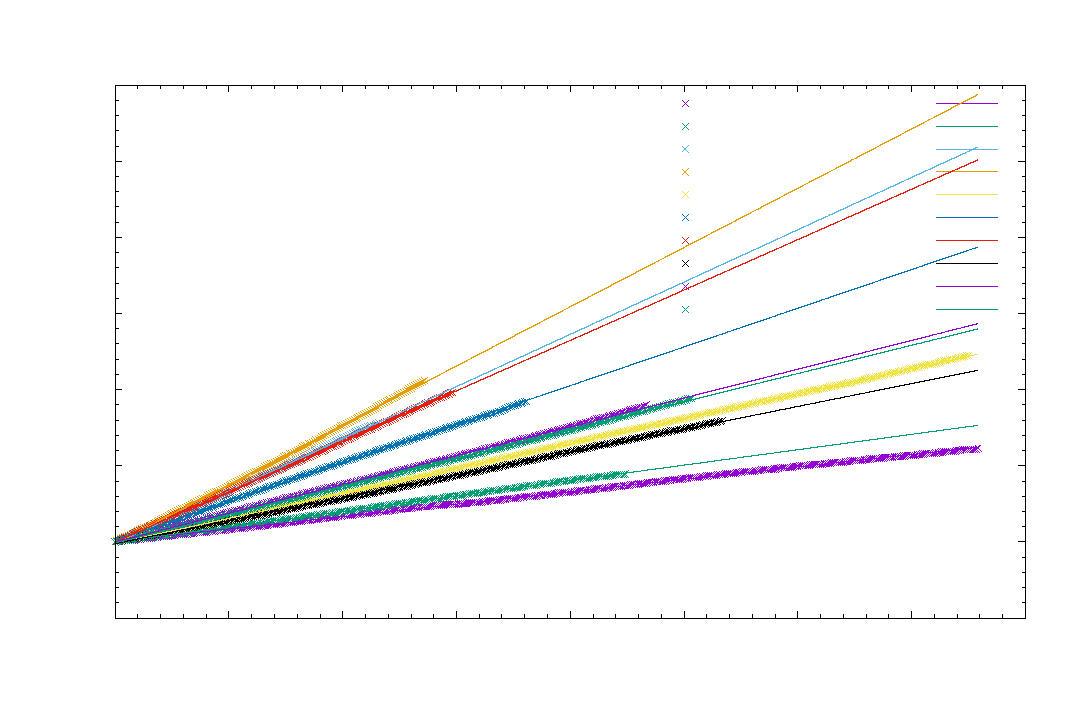
\includegraphics[width={504.00bp},height={324.00bp}]{tv1-plot-cold}}%
    \gplfronttext
  \end{picture}%
\endgroup
}
			\caption{Aufstieg der Luftblasen im kalten Spülmittel \textattachfile[author={Yudong Sun},color={0 0.404 0.584},description={.zip Datei mit der Messwerten},mimetype={application/zip},timezone={+02'00'}]{./attachments/luftblasen-kalt.zip}{\textit{(Daten)}}}
			\vspace{-1em}
		\end{figure}
		\newpage
		Als Endergebnis erhalten wir:
		\begin{center}
			\begin{tabular}{lrrr}
				\toprule
				Blase Nr. & $m/\si{\milli\meter\per\second}$ & $c/\si{\milli\meter}$ & $\chi^2_\text{red}$ \\
				\midrule
					$1$ & \num{8,15080(813)} & \num{0,34556(3560)} & \num{0,14495} \\
					$2$ & \num{10,12025(686)} & \num{-0,18451(1777)} & \num{0,02144} \\
					$3$ & \num{34,33273(4927)} & \num{-0,96333(6602)} & \num{0,15418} \\
					$4$ & \num{38,91436(6953)} & \num{-1,19706(10923)} & \num{0,49363} \\
					$5$ & \num{16,38475(854)} & \num{-0,93825(3701)} & \num{0,15491} \\
					$6$ & \num{25,41788(3870)} & \num{0,96616(8091)} & \num{0,35920} \\
					$7$ & \num{33,10418(2057)} & \num{-0,07643(3528)} & \num{0,05617} \\
					$8$ & \num{15,00664(1969)} & \num{-1,06078(6068)} & \num{0,29691} \\
					$9$ & \num{18,90101(1844)} & \num{0,01798(4973)} & \num{0,17465} \\
					$10$ & \num{18,54460(1597)} & \num{-0,69004(4676)} & \num{0,16751} \\
				\bottomrule
			\end{tabular}
		\end{center}
		Aus der niedrigen $\chi^2_\text{red}$ sind alle Kurveanpassungen gut. 

		\iu{Viskosität mittels LibreOffice Calc}

		Wir berechnen nun die Viskosität $\eta$ mittels \eqref{eqn:warm-eta} und \eqref{eqn:warm-delta-eta} in LibreOffice Calc:
		\begin{center}
			\begin{tabular}{lrrr}
				\toprule
				Blase Nr. $i$ & $2r_i/\si{\milli\meter}$ & $v_i/\si{\milli\meter\per\second}$ & $\eta_i/\si{\milli\pascal\second}$ \\
				\midrule
				\num{1} & \num{8.23(6)} & \num{8.151(9)} & \num{4890(290)} \\
				\num{2} & \num{8.05(5)} & \num{10.12(7)} & \num{3770(220)} \\
				\num{3} & \num{11.91(26)} & \num{34.33(5)} & \num{2430(180)} \\
				\num{4} & \num{13.73(27)} & \num{38.91(7)} & \num{2850(200)} \\
				\num{5} & \num{8.54(9)} & \num{16.385(9)} & \num{2620(160)} \\
				\num{6} & \num{9.76(5)} & \num{25.42(4)} & \num{2210(130)} \\
				\num{7} & \num{10.86(9)} & \num{33.104(21)} & \num{2100(130)} \\
				\num{8} & \num{8.93(9)} & \num{15.01(20)} & \num{3130(190)} \\
				\num{9} & \num{9.02(11)} & \num{18.901(19)} & \num{2530(160)} \\
				\num{10} & \num{9.09(6)} & \num{18.545(16)} & \num{2620(150)} \\
				\bottomrule
			\end{tabular}
		\end{center}
		und den Mittelwert, die Unsicherheit des Mittelwertes (mittels Gleichung \eqref{eqn:avg-eta-warm}) und die Standardabweichung (mittels Gleichung \eqref{eqn:stdev-eta-warm}) in LibreOffice Calc:
		\begin{center}
			\begin{tabular}{lrr}
				\toprule
				Mittelwert & $\overline{\eta}$ & \SI{2915}{\milli\pascal\second}\\
				Unsicherheit des Mittelwertes & $\Delta\overline{\eta}$ & \SI{60}{\milli\pascal\second}\\
				Standardabweichung & $s(\eta)$ & \SI{850}{\milli\pascal\second}\\
				\bottomrule
			\end{tabular}
		\end{center}
		wobei $\Delta\overline{\eta}$ und $s(\eta)$ beides auf 2 signifikanten Ziffern aufgerundet sind. 

		Da die Standardabweichung größer als die Unsicherheit des Mittelwertes ist, nehmen wir die Standardabweichung als Fehler. Da das Spülmittel am Anfang und am Ende unterschiedliche Temperaturen hat, berechnen wir nun den Mittelwert:
		\begin{align}
			T' &= \frac{\SI{4}{\celsius} + \SI{12}{\celsius}}{2} = \SI{8}{\celsius} \\
			\Delta T' &= \frac{1}{2} \addquadpure{\SI{1}{\celsius}, \SI{1}{\celsius}} = \SI{0.8}{\celsius}
		\end{align}

		 und erhalten für $T' = \SI{8.0(8)}{\celsius}$ eine Viskosität von $\eta = \SI{2900(900)}{\milli\pascal\second}$.

	\subsubsection{Diskussion}
		Zusammengefasst mit der Herstellerangabe zur Viskosität\footnote{\url{daten.oehme-lorito.de/sdb/frosch\%20geschirrsp\%C3\%BClmittel\%20limonen.pdf}, Seite 6} haben wir:
		\begin{center}
			\begin{tabular}{lrr}
				\toprule
				Quelle & Temperatur$/\si{\celsius}$ & Viskosität$/\si{\milli\pascal\second}$ \\
				\midrule
				Experiment & \num{29(1)} & \num{256(28)} \\
				Experiment & \num{8.0(8)} & \num{2900(900)} \\
				Hersteller & ca. \num{20} & \num{1000} \\
				\bottomrule
			\end{tabular}
		\end{center}
		Da die Fehler ziemlich groß war (11\% beim Warmen, 31\% beim Kalten), ist es nicht sehr aussagekräftig im dreifachen Fehlerintervall zu vergleichen. Wir vergleichen somit immer nur im einfachen Fehlerintervall der Werten. Die Fehler könnten kleiner sein, wenn wir statt der Standardabweichung, der Fehler der Steigung zur optimalen Gerade der folgenden Gleichung verwenden:
		\begin{equation}
			r^2_\text{Luftblase} = \left(\frac{2}{9g}\cdot \frac{\eta_\spuli}{\rho_\spuli}\right)v_\text{Luftblase} + c
		\end{equation}
		$\displaystyle \frac{\eta_\spuli}{\rho_\spuli}$ ist dabei die kinematische Viskosität.

		$c$ ist nur da, sodass die Kurveanpassung möglichst allgemein ist. Es soll eigentlich $0$ sein. 

		Die Viskosität des kalten Spülmittels ist deutlich größer als die Viskosität des warmen Spülmittels, was auch erwartet ist. Bei niedriger Temperaturen haben die Moleküle weniger kinetische Energie, somit brauchen die Moleküle mehr äußere Energie, um die elektrischen Kräfte zwischen benachbarten Teilchen zu überwinden.

		Die Viskosität des warmen Spülmittels stimmt aber nicht mit der Herstellerangabe überein. Dabei ist der experimentelle Wert kleiner als der Literaturwert. Es ist aber zu bemerken, dass die Temperatur beim Experiment auch deutlich höher als die Temperatur im Literatur. Ob es tatsächlich einen Fehler im Experiment gibt oder es einfach der Temperaturverlauf der Viskosität zurückzuführen ist, kann man ohne Zusatzexperiment schwer schlussfolgern. 

		Die Messung, die am stärksten zur Unsicherheit des Ergebnisses beiträgt, ist die Messung der Dichte des Spülmittels, da der prozentuale Fehler am größten ist. Ein systematische Fehler bei der Bestimmung ist die mögliche Verzerrung, die aus dem Objektiv und Winkel des Kameras entsteht. Bei verschiedenen Objektiven kann Längen unterschiedlich lang sein. Diese Verzerrung muss man durch die genaue Charakterisierung des Objektiv bestimmen, was hier aus zeitliche Gründen nicht gemacht war. 

		Die Reynoldszahl ist gegeben durch:
		\begin{align}
			R_e &= \frac{v\cdot 2r \cdot \rho_\spuli}{\eta_\spuli} \\
			\Delta R_e &= R_e \relquad{v, (2r), \rho_\spuli, \eta_\spuli}
		\end{align}
		Wir berechnen nun alle Reynoldszahlen mit Hilfe von LibreOffice Calc und nehmen an, dass die Dichte des Spülmittel nicht Temperaturabhängig ist. 
		\newpage
		Aus LibreOffice Calc gilt:
		\begin{center}
			\begin{tabular}{lrrrr}
				Warm \\
				\toprule
				Blase Nr. $i$ & $2r_i/\si{\milli\meter}$ & $v_i/\si{\milli\meter\per\second}$ & $\eta_i/\si{\milli\pascal\second}$ & $R_e$\\
				\midrule
				\num{1} & \num{2.84(7)} & \num{18.759(17)} & \num{253(19)} & \num{0.227(22)} \\
				\num{2} & \num{2.633(27)} & \num{14.881(4)} & \num{274(17)} & \num{0.154(13)} \\
				\num{3} & \num{3.04(6)} & \num{23.809(11)} & \num{228(16)} & \num{0.34(4)} \\
				\num{4} & \num{2.64(12)} & \num{14.788(8)} & \num{280(30)} & \num{0.152(20)} \\
				\num{5} & \num{3.49(6)} & \num{28.05(4)} & \num{256(17)} & \num{0.41(4)} \\
				\num{6} & \num{3.56(5)} & \num{35.18(2)} & \num{212(14)} & \num{0.64(6)} \\
				\num{7} & \num{7.11(26)} & \num{99.39(15)} & \num{299(28)} & \num{2.5(3)} \\
				\num{8} & \num{5.57(18)} & \num{67.19(9)} & \num{272(24)} & \num{1.49(17)} \\
				\num{9} & \num{2.75(12)} & \num{17.521(5)} & \num{254(27)} & \num{0.205(27)} \\
				\num{10} & \num{3.74(9)} & \num{36.195(9)} & \num{227(17)} & \num{0.64(7)} \\
				\bottomrule
				\\
				Kalt \\
				\toprule
				Blase Nr. $i$ & $2r_i/\si{\milli\meter}$ & $v_i/\si{\milli\meter\per\second}$ & $\eta_i/\si{\milli\pascal\second}$ & $R_e$\\
				\midrule
				\num{1} & \num{8.23(6)} & \num{8.151(9)} & \num{4890(290)} & \num{0.0148(13)} \\
				\num{2} & \num{8.05(5)} & \num{10.12(7)} & \num{3770(220)} & \num{0.0233(19)} \\
				\num{3} & \num{11.91(26)} & \num{34.33(5)} & \num{2430(180)} & \num{0.182(18)} \\
				\num{4} & \num{13.73(27)} & \num{38.91(7)} & \num{2850(200)} & \num{0.202(19)} \\
				\num{5} & \num{8.54(9)} & \num{16.385(9)} & \num{2620(160)} & \num{0.058(5)} \\
				\num{6} & \num{9.76(5)} & \num{25.42(4)} & \num{2210(130)} & \num{0.121(10)} \\
				\num{7} & \num{10.86(9)} & \num{33.104(21)} & \num{2100(130)} & \num{0.185(16)} \\
				\num{8} & \num{8.93(9)} & \num{15.01(20)} & \num{3130(190)} & \num{0.046(4)} \\
				\num{9} & \num{9.02(11)} & \num{18.901(19)} & \num{2530(160)} & \num{0.073(7)} \\
				\num{10} & \num{9.09(6)} & \num{18.545(16)} & \num{2620(150)} & \num{0.069(6)} \\
				\bottomrule
			\end{tabular}
		\end{center}
		Da alle Reynoldzahlen kleiner als $2000$ ist, ist die Strömung wirklich laminar. 
			